\documentclass[11pt]{article}
\usepackage[letterpaper,top=16mm,bottom=17mm,left=15mm,right=15mm,headheight=14pt,headsep=5mm,footskip=9mm]{geometry}
\usepackage{helvet}
\renewcommand{\familydefault}{\sfdefault}
\usepackage[T1]{fontenc}
\usepackage{tikz}
\usetikzlibrary{arrows.meta,calc}
\usepackage{fancyhdr}
\usepackage{array}
\usepackage{amsmath}
\setlength{\parindent}{0pt}
\setlength{\parskip}{3mm}
\pagestyle{fancy}
\fancyhf{}
\renewcommand{\headrulewidth}{0.35pt}
\renewcommand{\footrulewidth}{0pt}
\newcommand{\band}{Grades 2--5}
\newcommand{\packetid}{W63-S-v2}
\fancyhead[L]{\small Week 63 / Cards away from home / \band}
\fancyfoot[L]{\footnotesize Bellingham Math Circle / Week 63 / \packetid}
\fancyfoot[R]{\footnotesize\thepage}
\newcommand{\problem}[2]{\noindent\textbf{Problem #1:} #2\par}
\newcommand{\nextpage}[1]{\newpage\renewcommand{\band}{#1}}
\newcommand{\worklines}[1]{\foreach \i in {1,...,#1}{\par\noindent\rule{\linewidth}{0.2pt}\vspace{8mm}}}
% All geometry below is in millimetres unless a local diagram says otherwise.
\newcommand{\rowdraw}[4]{%
  % x offset, y offset, comma-separated homes, comma-separated cards.
  \foreach \h [count=\i from 0] in {#3}{%
    \node[font=\scriptsize] at ({#1+\i*12+6},{#2+3}) {\h};
    \draw[thin] ({#1+\i*12},{#2-10}) rectangle ++(12,10);
  }
  \foreach \c [count=\i from 0] in {#4}{%
    \node[font=\normalsize] at ({#1+\i*12+6},{#2-5}) {\c};
  }
}
\newcommand{\blankrows}[3]{%
  % number of rows per column, comma-separated homes, cell count.
  \begin{center}\begin{tikzpicture}[x=1mm,y=1mm]
  \pgfmathtruncatemacro{\last}{#1-1}
  \foreach \r in {0,...,\last}{%
    \rowdraw{0}{-\r*20}{#2}{}
    \rowdraw{97}{-\r*20}{#2}{}
  }
  \end{tikzpicture}\end{center}
}
\newcommand{\cyclefive}[2]{%
  % labels in cyclic order, radius in mm; arrow means card -> home.
  \foreach \v [count=\i from 0] in {#1}{%
    \node[circle,draw,fill=white,minimum size=6mm,inner sep=0pt,font=\small]
      (v\i) at ({90-72*\i}:#2) {\v};
  }
  \foreach \i/\j in {0/1,1/2,2/3,3/4,4/0}{\draw[-{Stealth[length=2mm]},thin] (v\i)--(v\j);}
}
\newcommand{\cyclesix}[2]{%
  \foreach \v [count=\i from 0] in {#1}{%
    \node[circle,draw,fill=white,minimum size=5.8mm,inner sep=0pt,font=\small]
      (v\i) at ({90-60*\i}:#2) {\v};
  }
  \foreach \i/\j in {0/1,1/2,2/3,3/4,4/5,5/0}{\draw[-{Stealth[length=1.8mm]},thin] (v\i)--(v\j);}
}
\newcommand{\cyclefour}[2]{%
  \foreach \v [count=\i from 0] in {#1}{%
    \node[circle,draw,fill=white,minimum size=6mm,inner sep=0pt,font=\small]
      (v\i) at ({90-90*\i}:#2) {\v};
  }
  \foreach \i/\j in {0/1,1/2,2/3,3/0}{\draw[-{Stealth[length=1.8mm]},thin] (v\i)--(v\j);}
}
\newcommand{\fourworkspace}[2]{%
  \begin{scope}[shift={(#1,#2)}]
    \rowdraw{-24}{28}{A,B,C,D}{}
    \foreach \v/\x/\y in {A/-17/8,B/17/8,C/17/-20,D/-17/-20}{%
      \node[circle,draw,fill=white,minimum size=6mm,inner sep=0pt,font=\small] at (\x,\y) {\v};}
  \end{scope}
}
\ifdefined\pdfinfoomitdate\pdfinfoomitdate=1\fi
\ifdefined\pdftrailerid\pdftrailerid{}\fi
\ifdefined\pdfsuppressptexinfo\pdfsuppressptexinfo=15\fi

\renewcommand{\band}{Materials}
\renewcommand{\packetid}{W63-M-v2}
\newcommand{\card}[3]{%
  \begin{scope}[shift={(#1,#2)}]
    \draw[thin] (0,0) rectangle (30,40);
    \node[font=\Large\bfseries] at (15,31) {#3};
    \begin{scope}[shift={(15,15)}]
    \if A#3\draw[fill=black!12] (0,0) circle (6mm);\fi
    \if B#3\draw[fill=black!12] (0,6.9282032303)--(-6,-3.4641016151)--(6,-3.4641016151)--cycle;\fi
    \if C#3\draw[fill=black!12] (-6,-6) rectangle (6,6);\fi
    \if D#3\draw[fill=black!12] (0,8.4852813742)--(8.4852813742,0)--(0,-8.4852813742)--(-8.4852813742,0)--cycle;\fi
    \if E#3\draw[fill=black!12] (90:8)\foreach \a/\r in {54/3.5,18/8,-18/3.5,-54/8,-90/3.5,-126/8,-162/3.5,-198/8,-234/3.5}{--(\a:\r)}--cycle;\fi
    \end{scope}
  \end{scope}
}
\newcommand{\homes}[1]{%
  \foreach \h [count=\i from 0] in {A,B,C,D,E}{%
    \draw[thin] (\i*35,#1) rectangle ++(35,45);
    \node[font=\small\bfseries] at ({\i*35+17.5},{#1+42.5}) {\h};
  }
}
\newcommand{\outcome}[6]{%
  % x, y, homes, cards, number of homes, persistent complete-row identifier.
  \begin{scope}[shift={(#1,#2)}]
    \draw[thin] (0,0) rectangle (56,27);
    \foreach \h [count=\i from 0] in {#3}{%
      \node[font=\scriptsize] at ({28-#5*4.5+\i*9+4.5},21) {\h};
      \draw[thin] ({28-#5*4.5+\i*9},7) rectangle ++(9,10);
    }
    \foreach \value [count=\idx from 0] in {#4}{%
      \node[font=\normalsize\bfseries] at ({28-#5*4.5+\idx*9+4.5},12) {\value};
    }
    \node[font=\scriptsize] at (28,3) {#6};
  \end{scope}
}
\begin{document}
Print at 100\%. Cut out the cards and whole home strips. Place cards below the home letters so both labels stay visible. For three or four cards, cover the unused homes.

\begin{center}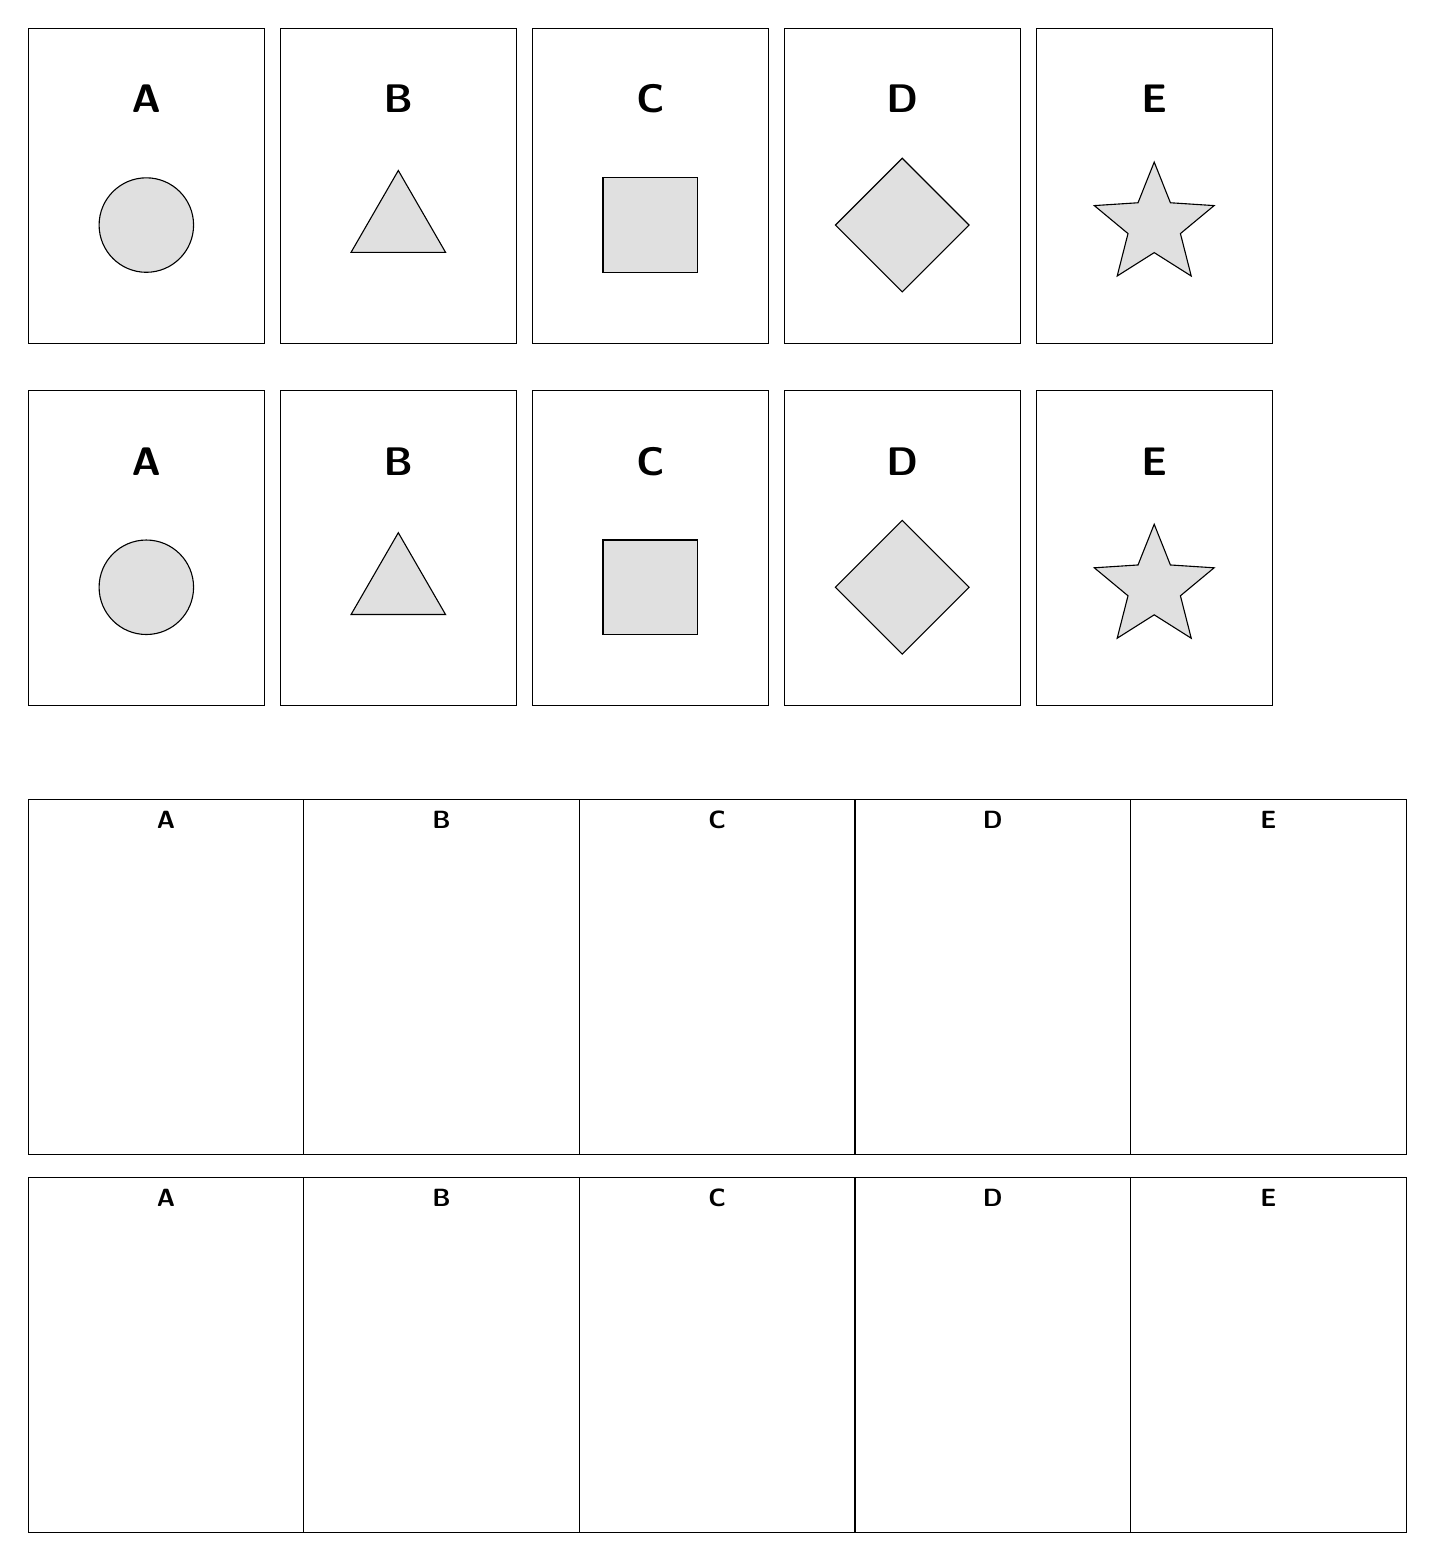
\begin{tikzpicture}[x=1mm,y=1mm]
  \foreach \h [count=\i from 0] in {A,B,C,D,E}{%
    \card{\i*32}{151}{\h}
    \card{\i*32}{105}{\h}
  }
  \homes{48}
  \homes{0}
\end{tikzpicture}\end{center}

\newpage
Cut out the six A--C outcomes and the group labels. Each outcome card is one complete placement. Blank A--E cards below can hold a shared catalog; print more copies as needed.

\begin{center}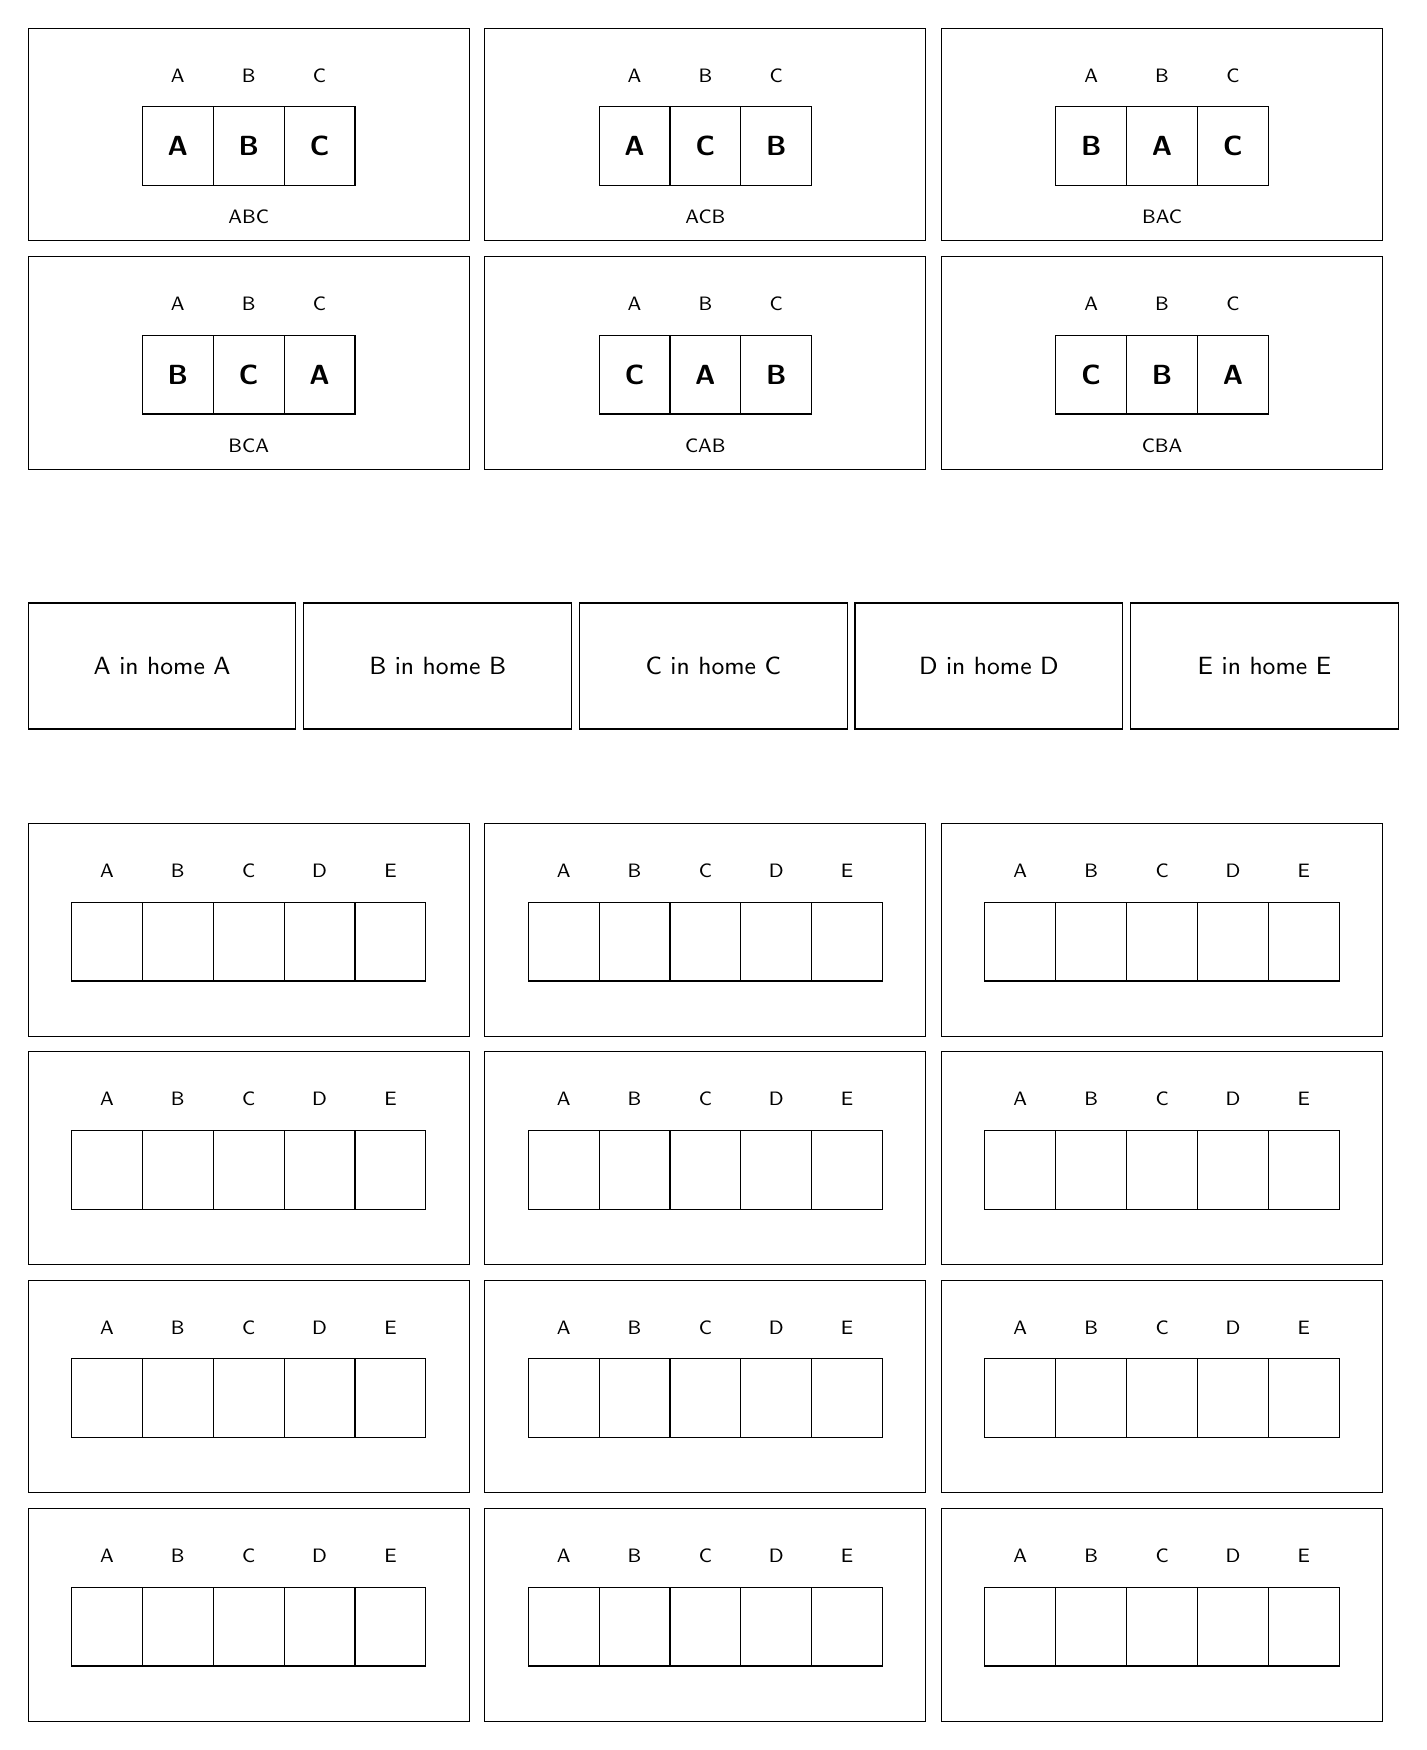
\begin{tikzpicture}[x=1mm,y=1mm]
  \foreach \a/\b/\c [count=\i from 0] in {A/B/C,A/C/B,B/A/C,B/C/A,C/A/B,C/B/A}{%
    \pgfmathtruncatemacro{\col}{mod(\i,3)}
    \pgfmathtruncatemacro{\r}{floor(\i/3)}
    \outcome{\col*58}{188-\r*29}{A,B,C}{\a,\b,\c}{3}{\a\b\c}
  }
  \foreach \i in {0,...,11}{%
    \pgfmathtruncatemacro{\col}{mod(\i,3)}
    \pgfmathtruncatemacro{\r}{floor(\i/3)}
    \outcome{\col*58}{87-\r*29}{A,B,C,D,E}{}{5}{}
  }
  \foreach \h [count=\i from 0] in {A,B,C,D,E}{%
    \draw[thin] (\i*35,126) rectangle ++(34,16);
    \node[font=\small] at ({\i*35+17},134) {\h\ in home \h};
  }
\end{tikzpicture}\end{center}

\newpage
Cut out the 24 A--D outcomes. Each card is one complete placement.

\begin{center}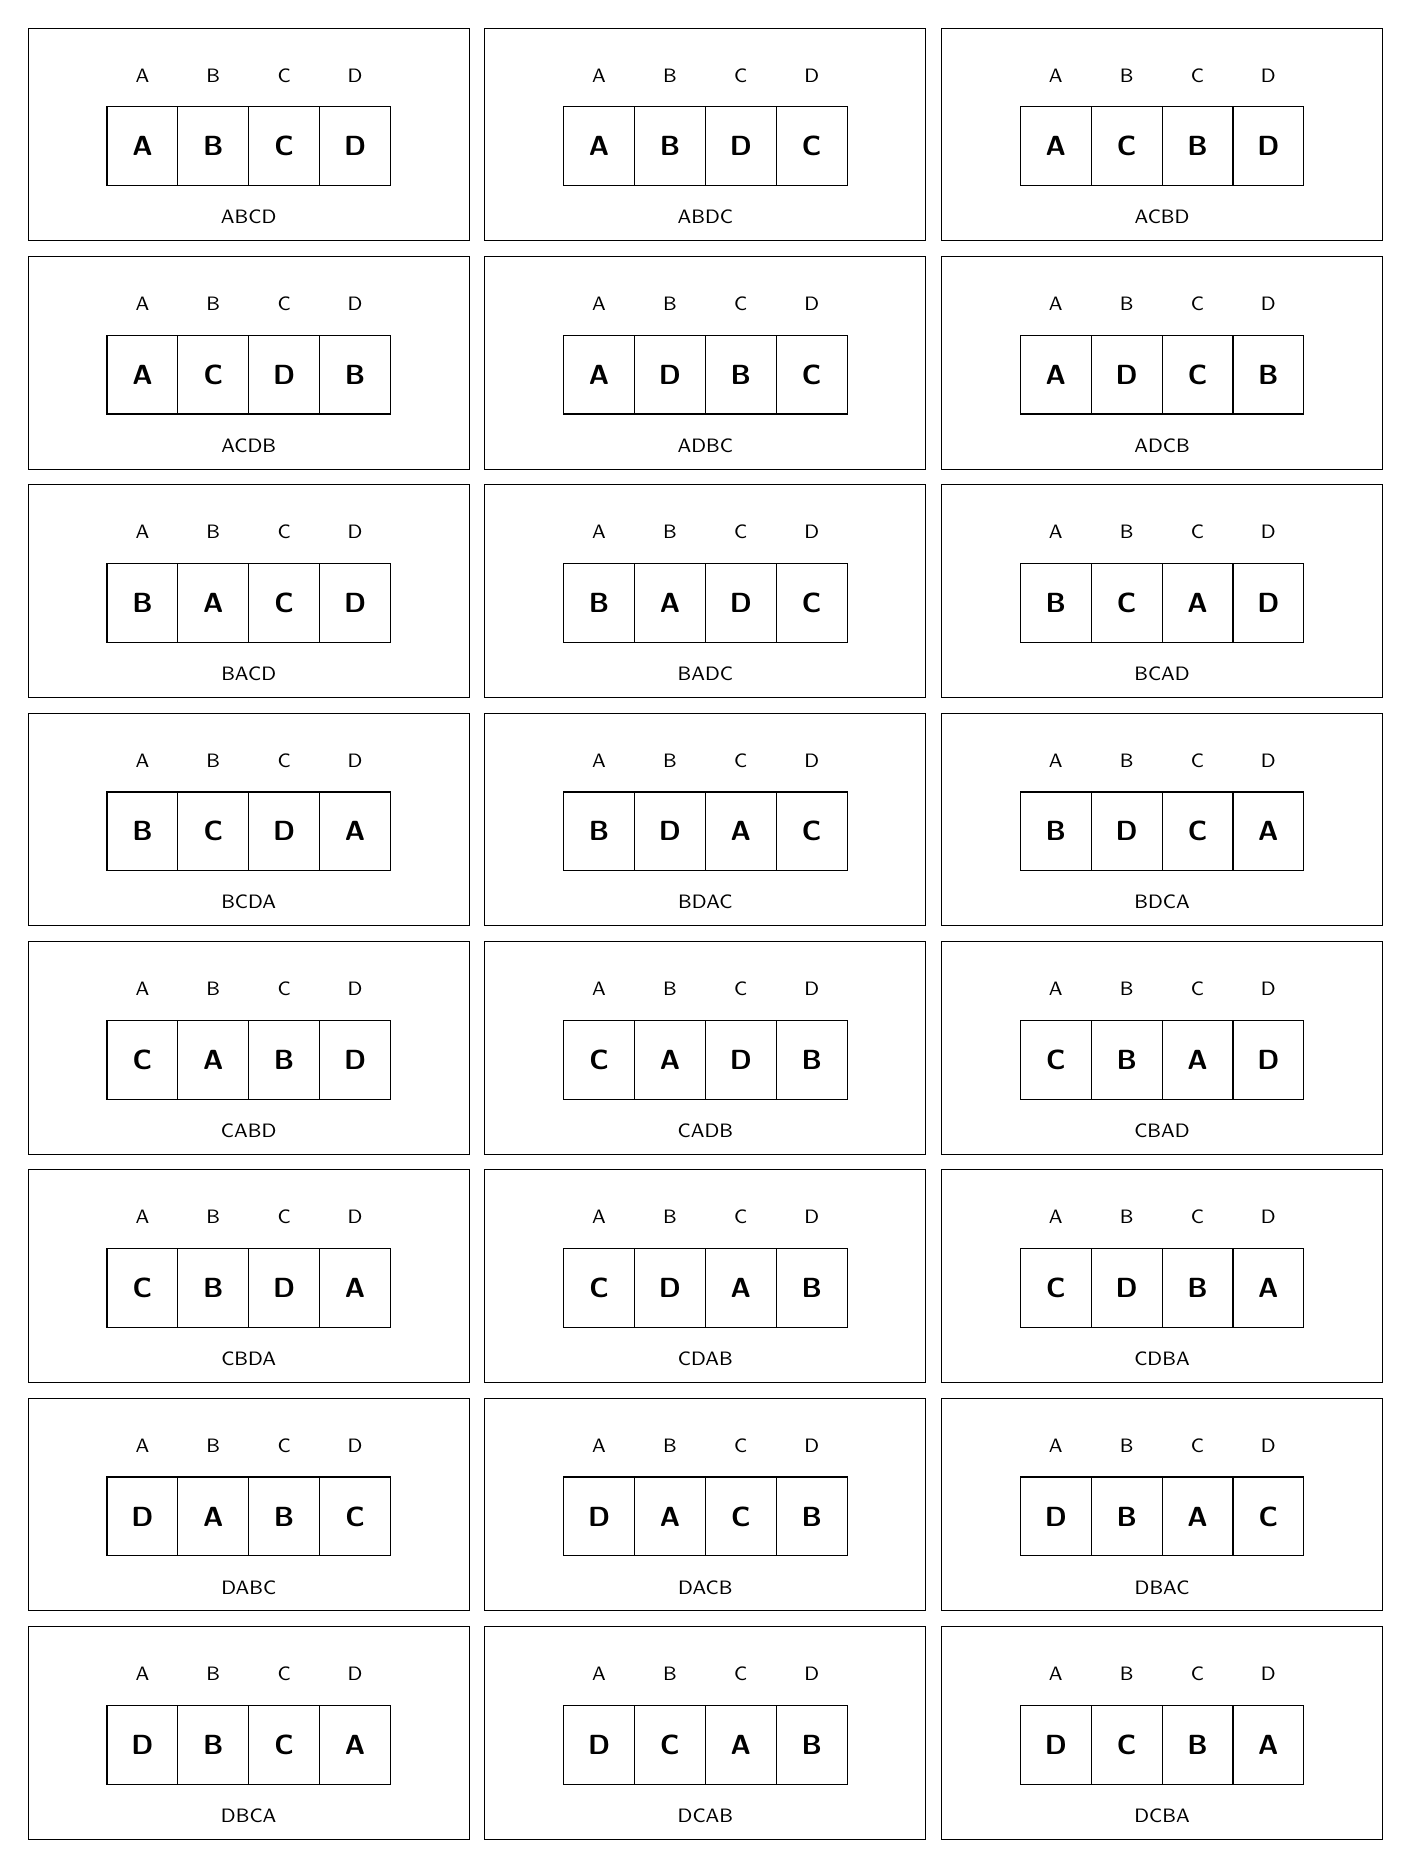
\begin{tikzpicture}[x=1mm,y=1mm]
  \foreach \a/\b/\c/\d [count=\i from 0] in {
    A/B/C/D,A/B/D/C,A/C/B/D,A/C/D/B,A/D/B/C,A/D/C/B,
    B/A/C/D,B/A/D/C,B/C/A/D,B/C/D/A,B/D/A/C,B/D/C/A,
    C/A/B/D,C/A/D/B,C/B/A/D,C/B/D/A,C/D/A/B,C/D/B/A,
    D/A/B/C,D/A/C/B,D/B/A/C,D/B/C/A,D/C/A/B,D/C/B/A}{%
    \pgfmathtruncatemacro{\col}{mod(\i,3)}
    \pgfmathtruncatemacro{\r}{floor(\i/3)}
    \outcome{\col*58}{203-\r*29}{A,B,C,D}{\a,\b,\c,\d}{4}{\a\b\c\d}
  }
\end{tikzpicture}\end{center}
\end{document}
